\documentclass[aspectratio=169,11pt]{ctexbeamer}

\usetheme{Madrid}
\usecolortheme{default}
\setbeamertemplate{navigation symbols}{}
\setbeamertemplate{footline}[frame number]

\usepackage{amsmath,amssymb,bm}
\usepackage{booktabs}
\usepackage{physics}
\usepackage{graphicx}
\usepackage{hyperref}

\title[\texorpdfstring{$^{171}$Yb effective CZ GRAPE}{171Yb effective CZ GRAPE}]%
{Shelving 后有效两能级 \texorpdfstring{$^{171}\mathrm{Yb}$}{171Yb} Rydberg CZ 的开放系统 phase-only GRAPE}
\subtitle{Notebook-first 开发报告：fidelity 与时序演化推导}
\author{Noise-Tolerant Quantum Control Optimization}
\date{\today}

\newcommand{\ketc}{\ket{c}}
\newcommand{\ketr}{\ket{r}}
\newcommand{\ketloss}{\ket{\mathrm{loss}}}
\newcommand{\OmegaMax}{\Omega_{\max}}
\newcommand{\Fpro}{F_{\mathrm{pro}}}
\newcommand{\Pact}{P_{\mathrm{active}}}
\newcommand{\Fgate}{F}

\begin{document}

\begin{frame}
  \titlepage
\end{frame}

\begin{frame}{本阶段目标}
  \begin{block}{Workflow 位置}
    这是三阶段 gated workflow 的第 2 阶段：在 notebook 原型通过后，记录模型、推导、数值结果和 artifact 路径。此阶段不集成 \texttt{src/} 代码。
  \end{block}

  \begin{itemize}
    \item 物理对象：参考 Muniz et al., PRX Quantum 6, 020334 (2025) 的 \({}^{171}\mathrm{Yb}\) clock shelving + UV Rydberg gate 图像。
    \item 简化目标：假设 shelving / unshelving 理想，只优化 shelving 后的 UV entangling segment。
    \item 控制约束：UV 振幅固定为 Gaussian 上下沿，plateau 为 \(\OmegaMax/2\pi=10\,\mathrm{MHz}\)，只优化相位 \(\phi(t)\)。
    \item 噪声：只加入 Rydberg 态 one-way decay，寿命 \(T_{1,r}=65\,\mu\mathrm{s}\)。
    \item 数值任务：扫描 UV segment time，寻找达到高 fidelity CZ 的最短时间。
  \end{itemize}
\end{frame}

\begin{frame}{Notebook 与输出}
  \begin{itemize}
    \item 开发 notebook：
      \[
      \texttt{notebooks/yb171\_effective\_two\_level\_cz\_time\_optimal\_grape.ipynb}
      \]
    \item JSON artifact：
      \[
      \texttt{artifacts/v5/effective\_two\_level\_cz\_time\_scan/}
      \]
      \[
      \texttt{yb171\_effective\_two\_level\_phase\_grape\_time\_scan.json}
      \]
    \item PNG artifact：
      \[
      \texttt{yb171\_effective\_two\_level\_phase\_grape\_time\_scan.png}
      \]
    \item 主要结果：粗扫中 \(F\ge 0.999\) 的最短点为 \(T_{\mathrm{UV}}=180\,\mathrm{ns}\)，
      \(F=0.9992514494\)。
  \end{itemize}
\end{frame}

\begin{frame}{完整门与本 notebook 的边界}
  \begin{columns}
    \begin{column}{0.52\textwidth}
      完整实验图像应分成 three coherent blocks：
      \[
      \begin{aligned}
      \ket{1}
      &\xrightarrow{\mathrm{shelving}}
      \ketc
      \xrightarrow{\mathrm{UV}:~\ketc\leftrightarrow\ketr}
      e^{i\varphi}\ketc,\\
      e^{i\varphi}\ketc
      &\xrightarrow{\mathrm{unshelving}}
      e^{i\varphi}\ket{1}.
      \end{aligned}
      \]
      也就是说，Rydberg population 必须由同一段 UV pulse coherently 打回 \(\ketc\)，
      然后才由 clock unshelving 回到逻辑 \(\ket{1}\)。
    \end{column}
    \begin{column}{0.44\textwidth}
      本 notebook 只优化中间 UV 段：
      \begin{itemize}
        \item 不模拟 clock pulse 误差；
        \item 不展开多个 \(m_F\) Rydberg 子能级；
        \item 不加入 Doppler / laser noise；
        \item 不加入 UV 振幅漂移；
        \item 只保留 Rydberg \(T_1\) decay。
      \end{itemize}
    \end{column}
  \end{columns}

  \vspace{0.8em}
  因此本 notebook 的目标不是优化 shelving / unshelving pulse，而是优化中间
  \(\ketc/\ketr\) UV 段的 unitary phase accumulation 和 Rydberg decay loss。
\end{frame}

\begin{frame}{Reduced basis}
  Shelving 后的 UV 段用 7 维 reduced basis：
  \[
  \begin{array}{ccl}
  0 &:& \ket{00},\\
  1 &:& \ket{01_c}\quad \text{代表 } \ket{01},\ket{10}\text{ 的单激发分支},\\
  2 &:& \ket{01_r},\\
  3 &:& \ket{11_{cc}},\\
  4 &:& \ket{11_{Wcr}},\\
  5 &:& \ket{11_{rr}},\\
  6 &:& \ketloss.
  \end{array}
  \]

  \[
  \ket{11_{Wcr}}=\frac{\ket{cr}+\ket{rc}}{\sqrt2}.
  \]

  active representative states:
  \[
  \{\ket{00},\ket{01_c},\ket{11_{cc}}\},
  \qquad
  w=(1,2,1).
  \]
  权重 \(2\) 表示 \(\ket{01}\) 与 \(\ket{10}\) 两条等价分支。
\end{frame}

\begin{frame}{Hamiltonian 结构}
  每个 time slot 内 Hamiltonian 视为常数：
  \[
  H_k=H_d+u_x(k)H_x+u_y(k)H_y.
  \]

  \[
  u_x(k)=A_k\cos\phi_k,\qquad
  u_y(k)=A_k\sin\phi_k.
  \]

  drift 只保留 double-Rydberg blockade：
  \[
  H_d = \frac{V}{\OmegaMax}\ket{11_{rr}}\bra{11_{rr}}.
  \]

  UV quadrature coupling:
  \[
  \ket{01_c}\leftrightarrow\ket{01_r}: \frac12,
  \]
  \[
  \ket{11_{cc}}\leftrightarrow\ket{11_{Wcr}}: \frac{1}{\sqrt2},
  \qquad
  \ket{11_{Wcr}}\leftrightarrow\ket{11_{rr}}: \frac{1}{\sqrt2}.
  \]
\end{frame}

\begin{frame}{单位和数值参数}
  \begin{table}
    \centering
    \begin{tabular}{lll}
      \toprule
      参数 & 数值 & notebook 中的无量纲形式 \\
      \midrule
      UV 最大 Rabi & \(10\,\mathrm{MHz}\) & \(\OmegaMax=1\) \\
      Blockade shift & \(160\,\mathrm{MHz}\) & \(V/\OmegaMax=16\) \\
      Rydberg lifetime & \(65\,\mu\mathrm{s}\) &
      \(\gamma_r=1/(\OmegaMax T_{1,r})\) \\
      Slot 数 & \(48\) & piecewise constant controls \\
      Edge envelope & Gaussian & edge fraction \(0.20\), sigma fraction \(0.08\) \\
      \bottomrule
    \end{tabular}
  \end{table}

  \[
  t_{\mathrm{dimless}}=\OmegaMax t_{\mathrm{physical}},
  \qquad
  \OmegaMax=2\pi\times 10\,\mathrm{MHz}.
  \]

  \[
  \gamma_r \simeq 2.4485\times 10^{-4}.
  \]
\end{frame}

\begin{frame}{Rydberg decay 的 Lindblad 形式}
  Rydberg decay 是 one-way loss：
  \[
  C_j=\sqrt{\gamma_j}\ketloss\bra{r_j}.
  \]

  对本 reduced basis：
  \[
  \gamma(\ket{01_r})=\gamma_r,\qquad
  \gamma(\ket{11_{Wcr}})=\gamma_r,\qquad
  \gamma(\ket{11_{rr}})=2\gamma_r.
  \]

  完整 Lindblad 方程为：
  \[
  \dot\rho=-i[H,\rho]
  +\sum_j C_j\rho C_j^\dagger
  -\frac12\sum_j\{C_j^\dagger C_j,\rho\}.
  \]

  由于 \(\ketloss\) 不回流到 active subspace，jump 项只增加 loss population，不向 active coherent block 反馈。
\end{frame}

\begin{frame}{投影定义与模型假设}
  设 \(P\) 是非 loss reduced Hilbert space 投影，包含 active \(\ketc\) branch
  和临时 Rydberg branch，但不含 \(\ketloss\)：
  \[
  \rho_P=P\rho P.
  \]

  设 \(Q=I-P\) 是 loss subspace 投影。当前 reduced model 满足：
  \[
  P\ketloss=0,\qquad Q\ketloss=\ketloss.
  \]

  Hamiltonian 不把 loss 态耦合回非 loss 子空间：
  \[
  PHQ=QHP=0.
  \]

  one-way decay jump operator 为：
  \[
  C_j=\sqrt{\gamma_j}\ketloss\bra{r_j},
  \qquad \ket{r_j}\in P.
  \]

  因此：
  \[
  PC_j=0,\qquad C_jP=C_j.
  \]
\end{frame}

\begin{frame}{Lindblad 方程逐项投影}
  完整 master equation:
  \[
  \dot\rho=-i[H,\rho]
  +\sum_j C_j\rho C_j^\dagger
  -\frac12\sum_j\{C_j^\dagger C_j,\rho\}.
  \]

  左右乘 \(P\)。Hamiltonian 项：
  \[
  P[H,\rho]P
  =
  [PHP,\,P\rho P].
  \]

  在本 reduced model 中 \(H\) 只作用在 \(P\) block，后面直接记作 \(H\)。

  jump feeding term:
  \[
  P C_j\rho C_j^\dagger P
  =
  (PC_j)\rho(C_j^\dagger P)
  =
  0.
  \]
\end{frame}

\begin{frame}{Lindblad 反对易项投影}
  定义 decay rate operator：
  \[
  \Gamma=\sum_j C_j^\dagger C_j.
  \]

  因为
  \[
  C_j^\dagger C_j=\gamma_j\ket{r_j}\bra{r_j},
  \]
  所以 \(\Gamma\) 完全位于 \(P\) block:
  \[
  P\Gamma P=\Gamma,\qquad Q\Gamma=\Gamma Q=0.
  \]

  于是反对易项投影为：
  \[
  P\{\Gamma,\rho\}P
  =
  \Gamma\rho_P+\rho_P\Gamma
  =
  \{\Gamma,\rho_P\}.
  \]

  因此 active / Rydberg block 的精确闭合方程是：
  \[
  \dot\rho_P
  =
  -i[H,\rho_P]-\frac12\{\Gamma,\rho_P\}.
  \]
\end{frame}

\begin{frame}{Active block 与 no-jump 生成元}
  定义 non-Hermitian Hamiltonian：
  \[
  H_{\mathrm{eff}}=H-\frac{i}{2}\Gamma,
  \]
  或 notebook 中直接使用 generator：
  \[
  G=-iH-\frac12\Gamma.
  \]

  则：
  \[
  \dot\rho_P
  =
  G\rho_P+\rho_P G^\dagger.
  \]

  这不是额外近似，而是上一页投影 Lindblad 方程的重写。
\end{frame}

\begin{frame}{Slot propagator 与密度矩阵解}
  第 \(k\) 个 time slot 中 \(H=H_k\)，因此：
  \[
  G_k=-iH_k-\frac12\Gamma.
  \]

  若 slot 内 \(G_k\) 常数，解为：
  \[
  \rho_P(t+\Delta t)
  =
  e^{\Delta t G_k}\rho_P(t)e^{\Delta t G_k^\dagger}.
  \]

  记第 \(k\) 个 slot 的 no-jump 传播矩阵为：
  \[
  M_k=e^{\Delta t G_k}.
  \]
\end{frame}

\begin{frame}{为什么可以传播 ket}
  若初始态在 \(P\) block 中是纯态：
  \[
  \rho_P(t)=\ket{\psi(t)}\bra{\psi(t)}.
  \]

  用上一页的密度矩阵解：
  \[
  \rho_P(t+\Delta t)
  =
  M_k\ket{\psi(t)}\bra{\psi(t)}M_k^\dagger.
  \]

  因此只要定义未归一化 ket：
  \[
  \ket{\psi(t+\Delta t)}=M_k\ket{\psi(t)},
  \]
  就有：
  \[
  \rho_P(t+\Delta t)=\ket{\psi(t+\Delta t)}\bra{\psi(t+\Delta t)}.
  \]

  notebook 的 ket propagation 正是在计算这个 \(P\) block 的精确 Lindblad 解。
\end{frame}

\begin{frame}{多段 pulse 的等价性}
  对 \(N\) 个 piecewise-constant slots，递推得到：
  \[
  M(T)=M_{N-1}M_{N-2}\cdots M_0.
  \]

  因此：
  \[
  \rho_P(T)=M(T)\rho_P(0)M(T)^\dagger.
  \]

  若从代表性初态 \(\ket{i}\) 出发：
  \[
  \ket{\psi_i(T)}=M(T)\ket{i}.
  \]

  回到目标逻辑态的 coherent amplitude 是：
  \[
  z_i=\bra{i}M(T)\ket{i}.
  \]

  这个 \(z_i\) 与直接解 Lindblad 方程后读取
  \(P\)-block matrix element 完全一致。
\end{frame}

\begin{frame}{与完整 Lindblad 解的关系}
  记 \(M(t)\) 为从初始时刻传播到时间 \(t\) 的 no-jump slot 矩阵乘积。

  对纯态初值 \(\rho_P(0)=\ket{\psi_0}\bra{\psi_0}\)，等价于传播未归一化 ket：
  \[
  \ket{\psi_P(t)}=M(t)\ket{\psi_0}.
  \]

  若初始态没有 loss coherence，完整 Lindblad 解还包含 loss block：
  \[
  \rho(t)=\rho_P(t)+\rho_{\mathrm{loss}}(t).
  \]

  当前 fidelity 只投影回逻辑 active output；\(\rho_{\mathrm{loss}}\) 与目标
  CZ 输出正交，所以不进入 trace-overlap numerator。

  也就是说，当前时序演化逻辑等价于完整 Lindblad 解在非 loss block 上的精确解；
  对本 fidelity，完整解的其余部分只表现为 active norm 的减少。
\end{frame}

\begin{frame}{Loss probability bookkeeping}
  loss block 记为
  \[
  \rho_{\mathrm{loss}}=(I-P)\rho(I-P).
  \]

  完整 density matrix 的 loss population 仍由 jump term 给出：
  \[
  \frac{d}{dt}\mathrm{Tr}\rho_{\mathrm{loss}}
  =
  \mathrm{Tr}(\Gamma\rho_P).
  \]

  no-jump ket 的 norm 正好给出未发生 loss 且仍在 \(P\) block 的概率：
  \[
  \frac{d}{dt}\mathrm{Tr}\rho_P
  =
  -\mathrm{Tr}(\Gamma\rho_P).
  \]
\end{frame}

\begin{frame}{这个等价性的适用范围}
  当前 fidelity 只投影回逻辑 active output；所有 jump trajectory 最终在
  \(\ketloss\)，与目标 CZ 逻辑输出正交，所以对 fidelity numerator 没有贡献。

  若 decay 回到会再被 pulse 耦合的态、或存在 dephasing / Raman scattering 到逻辑态，
  就必须保留完整 Lindblad / Kraus 集合，不能只用这个 no-jump propagator。
\end{frame}

\begin{frame}{active fidelity 只需要哪些 amplitude}
  对三个 representative initial states：
  \[
  \ket{i}\in
  \{\ket{00},\ket{01_c},\ket{11_{cc}}\}.
  \]

  前面已经定义了单段 no-jump 传播矩阵 \(M_k\)。整段 UV pulse 的 no-jump
  传播矩阵记为：
  \[
  M(T)=M_{N-1}M_{N-2}\cdots M_0.
  \]

  逻辑输出投影 \(P_L\) 只保留
  \(\{\ket{00},\ket{01_c},\ket{11_{cc}}\}\)，定义：
  \[
  K=P_LM(T)P_L.
  \]

  当前 Hamiltonian 不混合不同 computational branch，所以 \(K\) 在此 reduced basis 上近似为 diagonal；
  notebook 取：
  \[
  z_i=\bra{i}K\ket{i}
  =
  \bra{i}M(T)\ket{i}.
  \]

  \(z_i\) 同时包含相位误差、coherent return amplitude 和 decay/leakage 后的 survival。
\end{frame}

\begin{frame}{从四维逻辑空间到 reduced 权重}
  完整逻辑基是：
  \[
  \{\ket{00},\ket{01},\ket{10},\ket{11}\},
  \qquad d=4.
  \]

  目标 CZ 在这四维逻辑基中的 diagonal 元素记为：
  \[
  U_{\mathrm{tar}}=\mathrm{diag}(u_{00},u_{01},u_{10},u_{11}).
  \]

  shelving 后 \(\ket{01}\) 和 \(\ket{10}\) 对称，因此：
  \[
  z_{00}=z_0,\qquad
  z_{01}=z_{10}=z_1,\qquad
  z_{11}=z_2.
  \]

  所以完整四维 trace 可写成 reduced weighted trace：
  \[
  \mathrm{Tr}(U_{\mathrm{tar}}^\dagger K)
  =
  \sum_{\alpha\in\{00,01,10,11\}}
  u_\alpha^* z_\alpha
  =
  \sum_{i=0}^{2} w_i u_i^* z_i,
  \]
  其中：
  \[
  w=(1,2,1).
  \]
\end{frame}

\begin{frame}{目标 CZ 相位和可补偿相位}
  目标 reduced CZ phase 写作：
  \[
  u_0=e^{i\theta_0},
  \]
  \[
  u_1=e^{i(\theta_0+\theta_1)},
  \]
  \[
  u_2=-e^{i(\theta_0+2\theta_1)}.
  \]

  \(\theta_0,\theta_1\) 是优化变量：
  \begin{itemize}
    \item \(\theta_0\)：global phase；
    \item \(\theta_1\)：single-qubit phase；
    \item 负号：CZ 的 entangling phase。
  \end{itemize}

  这样 fidelity 不惩罚可通过单比特 \(Z\) phase frame 补偿的相位。
\end{frame}

\begin{frame}{Process fidelity 的推导：Kraus 形式}
  对一般开放系统逻辑通道：
  \[
  \mathcal{E}(\rho)=\sum_\mu K_\mu\rho K_\mu^\dagger.
  \]

  相对于目标 unitary \(U_{\mathrm{tar}}\)，entanglement / process fidelity 为：
  \[
  \Fpro=
  \frac{1}{d^2}
  \sum_\mu
  \left|\mathrm{Tr}(U_{\mathrm{tar}}^\dagger K_\mu)\right|^2.
  \]

  当前 noise 只有 one-way loss。所有 jump Kraus 都把态送到 loss subspace，
  投影回逻辑输出后 trace overlap 为零。因此只有 no-jump logical Kraus
  \[
  K=P_LM(T)P_L
  \]
  对 \(\Fpro\) 有贡献。

  代入 reduced diagonal / symmetry 近似得到：
  \[
  \Fpro=
  \frac{\left|\sum_i w_i u_i^*z_i\right|^2}{16}.
  \]
\end{frame}

\begin{frame}{Active population 与平均 gate fidelity}
  一般 CP map 的 Haar average gate fidelity 是：
  \[
  F_{\mathrm{avg}}
  =
  \frac{
  \sum_\mu\mathrm{Tr}(K_\mu^\dagger K_\mu)
  +
  \sum_\mu|\mathrm{Tr}(U_{\mathrm{tar}}^\dagger K_\mu)|^2
  }{d(d+1)}.
  \]

  定义 average active survival：
  \[
  \Pact
  =
  \frac{\sum_i w_i |z_i|^2}{4}.
  \]

  在 \(d=4\) 且只有 no-jump Kraus 对逻辑输出有贡献时：
  \[
  F_{\mathrm{avg}}
  =
  \frac{4\Fpro+\Pact}{5}.
  \]

  所以 notebook 中的 \(F\) 应理解为当前 projected logical open-system average gate fidelity；
  它不是单独的 process fidelity，也不是单独的 survival probability。
\end{frame}

\begin{frame}{时序演化实现}
  每个 slot：
  \[
  G_k=-iH_k-\frac12\Gamma,
  \qquad
  \Gamma=\sum_j C_j^\dagger C_j.
  \]

  piecewise-constant propagator：
  \[
  M_k=\exp(\Delta t\,G_k).
  \]

  总传播：
  \[
  M(T)=M_{N-1}\cdots M_1 M_0.
  \]

  对每个 representative 初态单独传播：
  \[
  \ket{\psi_i^{(k+1)}}=M_k\ket{\psi_i^{(k)}}.
  \]

  最终：
  \[
  z_i=\bra{i}M(T)\ket{i}.
  \]
\end{frame}

\begin{frame}{为什么这个 fidelity 与时序演化匹配}
  当前模型假设：
  \begin{itemize}
    \item no return from \(\ketloss\)；
    \item active 目标只关心 diagonal CZ phase；
    \item computational branches 不互相混合，\(K\) 可由 \(z_i\) 的 diagonal 元素表示；
    \item \(\ket{01}\) 与 \(\ket{10}\) 对称，用权重 \(2\) 表示。
  \end{itemize}

  时序演化给出：
  \[
  K=P_LM(T)P_L,\qquad z_i=\bra{i}K\ket{i}.
  \]

  master equation 的 jump trajectories 最终落在 loss subspace，与 \(U_{\mathrm{tar}}\ket{i}\) 正交；
  因而 fidelity 的相干 trace overlap 和 active survival 都可由 \(K\) 的这些元素计算：
  \[
  \Fgate=\frac{4\Fpro+\Pact}{5}.
  \]
\end{frame}

\begin{frame}{GRAPE 优化变量}
  固定振幅 envelope：
  \[
  A_k\in[0,1],
  \]
  前后 Gaussian edge，中间 plateau 为 \(1\)。

  优化变量：
  \[
  \bm{x}=(\phi_0,\ldots,\phi_{N-1},\theta_0,\theta_1).
  \]

  控制：
  \[
  u_x(k)=A_k\cos\phi_k,
  \qquad
  u_y(k)=A_k\sin\phi_k.
  \]

  objective：
  \[
  J(\bm{x})=1-\Fgate+\lambda_1 R_{\mathrm{smooth}}+\lambda_2 R_{\mathrm{curv}}.
  \]

  优化器：SciPy \texttt{L-BFGS-B}。
\end{frame}

\begin{frame}{GRAPE 梯度：单段导数}
  对 slot \(k\)：
  \[
  G_\alpha=\frac{\partial G_k}{\partial u_\alpha(k)}
  =
  -iH_\alpha,
  \qquad
  \alpha\in\{x,y\}.
  \]

  因此单段传播矩阵 \(M_k=\exp(\Delta tG_k)\) 的导数为：
  \[
  \frac{\partial M_k}{\partial u_\alpha(k)}
  =
  \mathcal{L}_{\exp}
  \left(\Delta t\,G_k,\Delta t\,G_\alpha\right).
  \]

  notebook 中使用：
  \[
  \texttt{scipy.linalg.expm\_frechet}.
  \]
\end{frame}

\begin{frame}{GRAPE 梯度：链式传播}
  prefix / suffix 链式传播：
  \[
  \frac{\partial z_i}{\partial u_\alpha(k)}
  =
  \bra{i}
  M_{N-1}\cdots M_{k+1}
  \frac{\partial M_k}{\partial u_\alpha(k)}
  M_{k-1}\cdots M_0
  \ket{i}.
  \]

  再由
  \[
  \frac{\partial u_x}{\partial\phi_k}=-A_k\sin\phi_k,\qquad
  \frac{\partial u_y}{\partial\phi_k}=A_k\cos\phi_k
  \]
  得到相位梯度。
\end{frame}

\begin{frame}{时间扫描设置}
  \begin{itemize}
    \item UV times:
      \[
      60,80,100,125,150,180,220,260,300\,\mathrm{ns}.
      \]
    \item Slot 数：\(N=48\)。
    \item 每个时间点：
      \begin{itemize}
        \item chirped phase seed；
        \item 上一个时间点 warm start；
        \item 3 个随机 phase seed；
        \item 取 fidelity 最高者。
      \end{itemize}
    \item 梯度检查：finite difference 最大误差约
      \[
      2.8\times10^{-10}.
      \]
  \end{itemize}
\end{frame}

\begin{frame}{时间扫描结果}
  \begin{table}
    \centering
    \small
    \begin{tabular}{rrrr}
      \toprule
      \(T_{\mathrm{UV}}\) [ns] & \(F\) & \(\Fpro\) & \(\Pact\) \\
      \midrule
       60 & 0.609820902 & 0.513092239 & 0.996735556 \\
       80 & 0.670310313 & 0.600435602 & 0.949809156 \\
      100 & 0.774223784 & 0.747721926 & 0.880231219 \\
      125 & 0.901940171 & 0.899685993 & 0.910956885 \\
      150 & 0.993898190 & 0.993873029 & 0.993998831 \\
      180 & 0.999251449 & 0.999251431 & 0.999251523 \\
      220 & 0.999123460 & 0.999123426 & 0.999123597 \\
      260 & 0.998951235 & 0.998951161 & 0.998951531 \\
      300 & 0.999094560 & 0.999094054 & 0.999096585 \\
      \bottomrule
    \end{tabular}
  \end{table}

  粗扫中首个达到 \(F\ge0.999\) 的时间为 \(180\,\mathrm{ns}\)。
\end{frame}

\begin{frame}{Artifact 图}
  \centering
  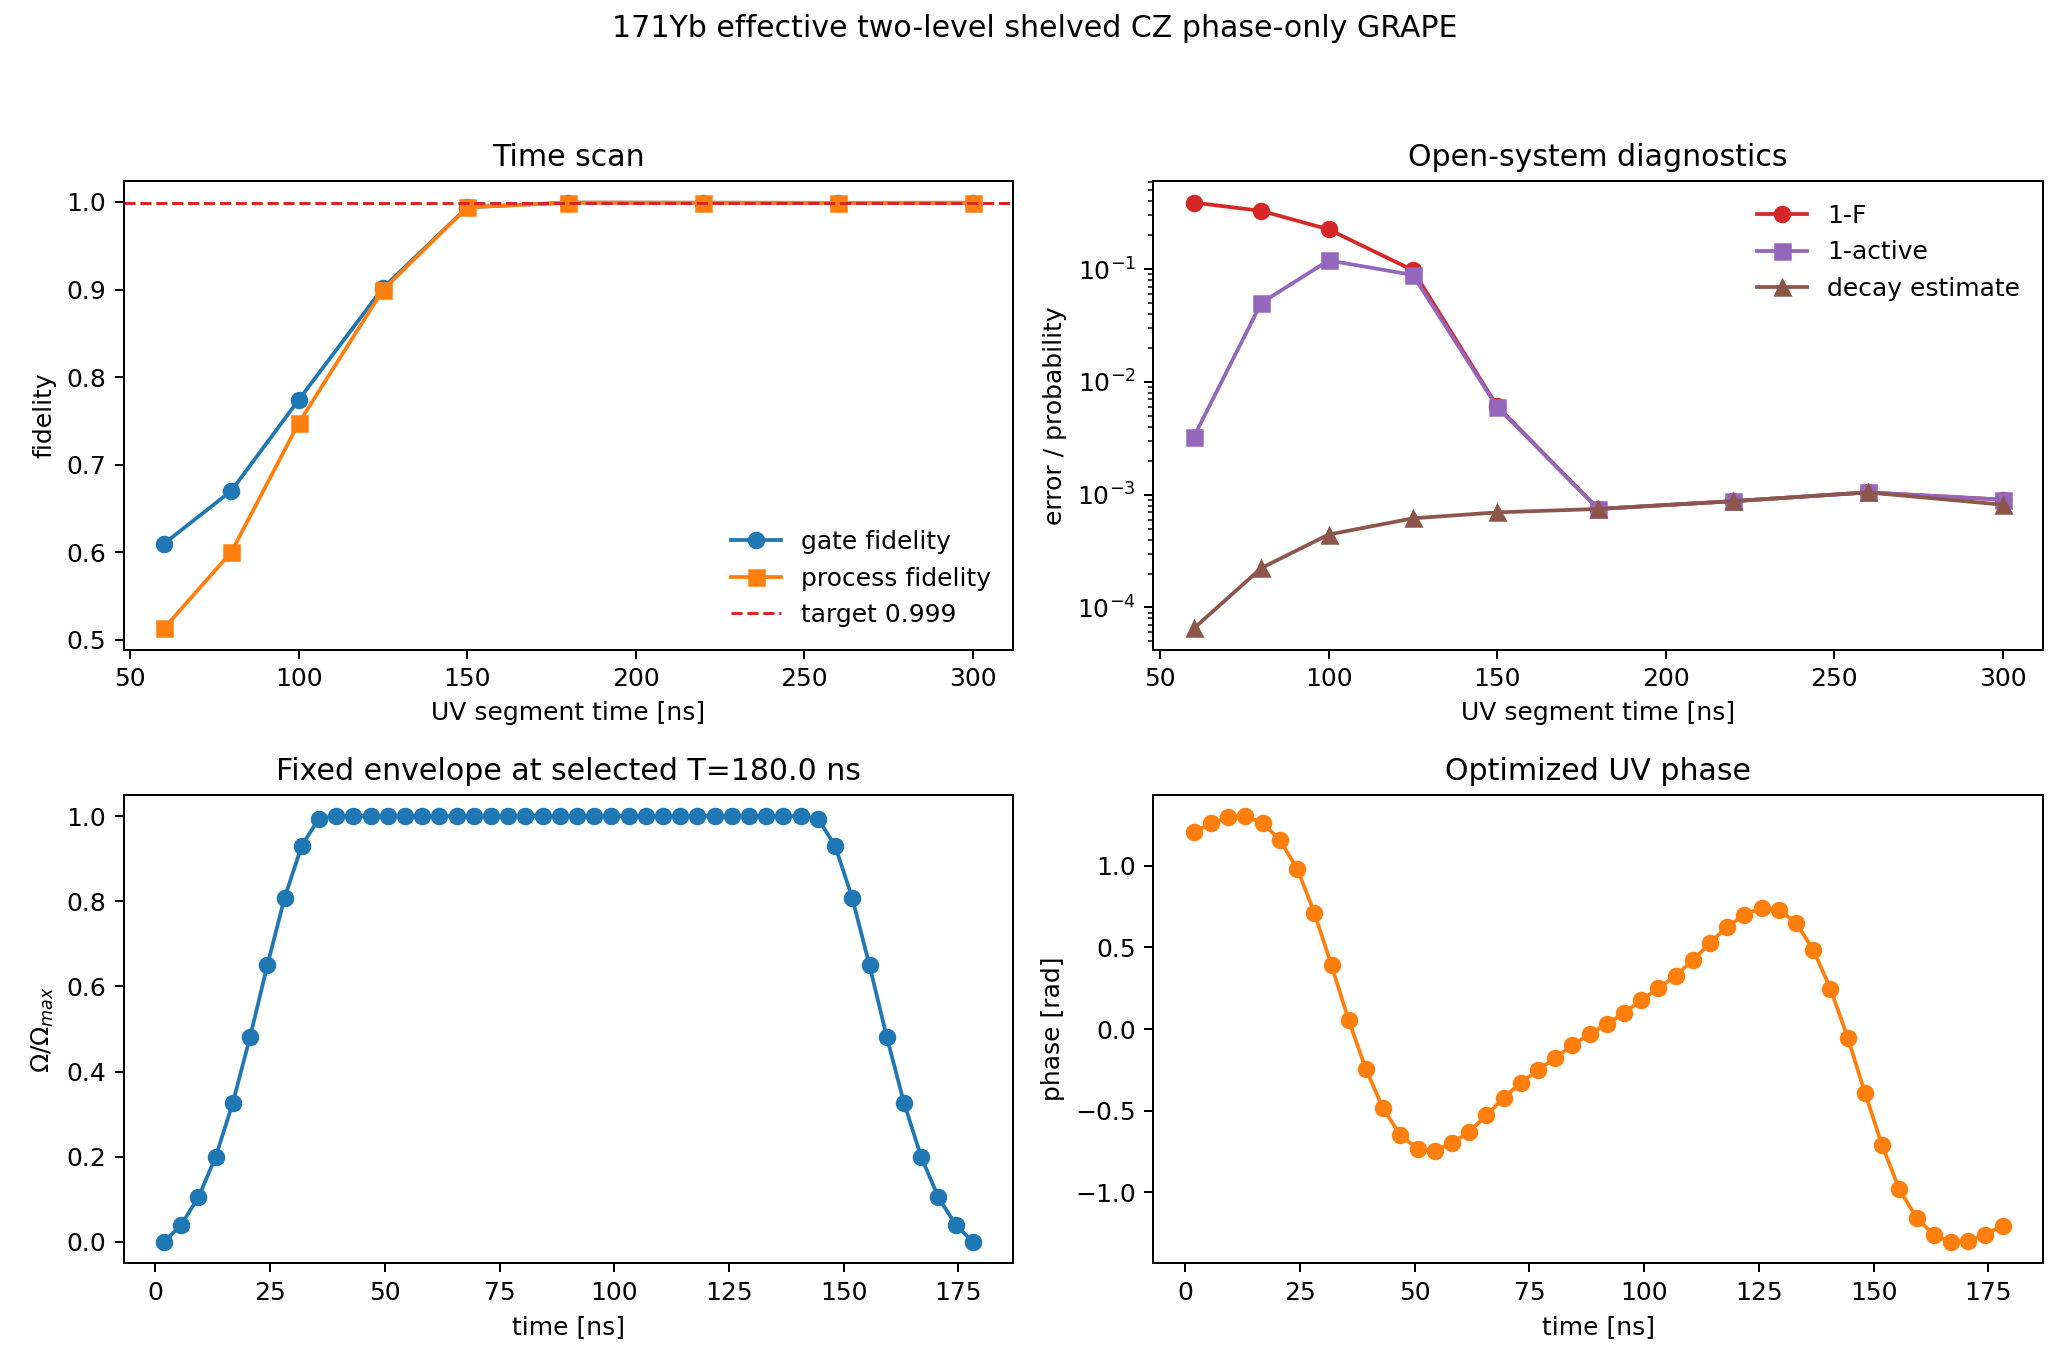
\includegraphics[width=0.92\linewidth,height=0.78\textheight,keepaspectratio]{../../artifacts/v5/effective_two_level_cz_time_scan/yb171_effective_two_level_phase_grape_time_scan.png}
\end{frame}

\begin{frame}{结果解读}
  \begin{itemize}
    \item \(150\,\mathrm{ns}\) 已达到 \(F\simeq0.9939\)，但未过 \(0.999\) 阈值。
    \item \(180\,\mathrm{ns}\) 达到 \(F\simeq0.999251\)，是当前粗扫最短达标点。
    \item \(180\)--\(300\,\mathrm{ns}\) 的 fidelity 差异较小，说明还需要更密时间网格和更多 seed 确认真正最短时间。
    \item Rydberg decay estimate 量级约 \(10^{-4}\)--\(10^{-3}\)，当前限制主要来自可达相位/泄漏优化，而不是单纯寿命误差。
  \end{itemize}
\end{frame}

\begin{frame}{当前限制}
  \begin{itemize}
    \item 只模拟 UV entangling segment；clock shelving / unshelving 被视为理想。
    \item 只保留有效两能级 Rydberg 模型；未展开邻近 \(m_F\) Rydberg 子能级。
    \item 只加入 Rydberg \(T_1\) decay；未加入 Doppler、laser phase noise、intensity noise、dephasing、finite temperature blockade jitter。
    \item 当前时间扫描是 notebook-scale 粗扫，不是最终 time-optimal benchmark。
    \item 使用 weighted diagonal reduced objective；后续集成前应增加 QuTiP Lindblad 正向验证和更严格 process-channel benchmark。
  \end{itemize}
\end{frame}

\begin{frame}{下一阶段建议}
  若本报告通过审查，进入第 3 阶段前建议明确：
  \begin{enumerate}
    \item 是否接受当前 reduced objective：
      \[
      F=(4\Fpro+\Pact)/5.
      \]
    \item 是否将 \(F\ge0.999\) 作为默认 threshold，还是改为 \(0.9999\) 或其他目标。
    \item 是否在 notebook 里先补更密扫描：
      \[
      140\text{--}200\,\mathrm{ns}
      \]
      多 seed、多 slot 数、更多迭代。
    \item 是否增加 QuTiP \texttt{mesolve} 正向验证作为 notebook 附录。
  \end{enumerate}

  只有审查通过后，才将优化器整理进 \texttt{src/neutral\_yb/optimization/}。
\end{frame}

\begin{frame}{参考文献}
  \begin{itemize}
    \item Muniz et al., PRX Quantum \textbf{6}, 020334 (2025), DOI:
      \href{https://doi.org/10.1103/PRXQuantum.6.020334}{10.1103/PRXQuantum.6.020334}.
    \item Notebook:
      \texttt{notebooks/yb171\_effective\_two\_level\_cz\_time\_optimal\_grape.ipynb}.
    \item Artifact JSON / PNG:
      \texttt{artifacts/v5/effective\_two\_level\_cz\_time\_scan/}.
  \end{itemize}
\end{frame}

\end{document}
